% This example is meant to be compiled with lualatex or xelatex
% The theme itself also supports pdflatex
\PassOptionsToPackage{unicode}{hyperref}
\documentclass[aspectratio=1610, 12pt]{beamer}

% Warning, if another latex run is needed
% \usepackage[aux]{rerunfilecheck}

% just list chapters and sections in the toc, not subsections or smaller
\setcounter{tocdepth}{1}

%------------------------------------------------------------------------------
%------------------------------ Fonts, Unicode, Language ----------------------
%------------------------------------------------------------------------------
\usepackage{fontspec}
\defaultfontfeatures{Ligatures=TeX}  % -- becomes en-dash etc.

% german language
\usepackage{polyglossia}
\setdefaultlanguage{german}

% for english abstract and english titles in the toc
\setotherlanguages{english}

% intelligent quotation marks, language and nesting sensitive
\usepackage[autostyle]{csquotes}

% microtypographical features, makes the text look nicer on the small scale
\usepackage{microtype}

%------------------------------------------------------------------------------
%------------------------ Math Packages and settings --------------------------
%------------------------------------------------------------------------------

\usepackage{amsmath}
\usepackage{amssymb}
\usepackage{mathtools}
\usepackage{bbold}

% Enable Unicode-Math and follow the ISO-Standards for typesetting math
\usepackage[
  math-style=ISO,
  bold-style=ISO,
  sans-style=italic,
  nabla=upright,
  partial=upright,
]{unicode-math}
\setmathfont{Latin Modern Math}

% nice, small fracs for the text with \sfrac{}{}
\usepackage{xfrac}


%------------------------------------------------------------------------------
%---------------------------- Numbers and Units -------------------------------
%------------------------------------------------------------------------------

\usepackage[
  locale=DE,
  separate-uncertainty=true,
  per-mode=symbol-or-fraction,
]{siunitx}
\sisetup{math-micro=\text{µ},text-micro=µ}
% \sisetup{tophrase={{ to }}}
%------------------------------------------------------------------------------
%-------------------------------- tables  -------------------------------------
%------------------------------------------------------------------------------

\usepackage{booktabs}       % \toprule, \midrule, \bottomrule, etc

%------------------------------------------------------------------------------
%-------------------------------- graphics -------------------------------------
%------------------------------------------------------------------------------

\usepackage{graphicx}
%\usepackage{rotating}
\usepackage{grffile}
\usepackage{tikz}
\usepackage{circuitikz}
\usepackage{tikz-feynman}
\usepackage{subcaption}

% allow figures to be placed in the running text by default:
\usepackage{scrhack}
\usepackage{float}
\floatplacement{figure}{htbp}
\floatplacement{table}{htbp}

% keep figures and tables in the section
\usepackage[section, below]{placeins}

% smileys
\usepackage{MnSymbol,wasysym}

%------------------------------------------------------------------------------
%---------------------- customize list environments ---------------------------
%------------------------------------------------------------------------------

\usepackage{enumitem}
\usepackage{listings}
\usepackage{hepunits}

\usepackage{pdfpages}
%------------------------------------------------------------------------------
%------------------------------ Bibliographie ---------------------------------
%------------------------------------------------------------------------------

\usepackage[
  backend=biber,   % use modern biber backend
  autolang=hyphen, % load hyphenation rules for if language of bibentry is not
                   % german, has to be loaded with \setotherlanguages
                   % in the references.bib use langid={en} for english sources
]{biblatex}
\addbibresource{references.bib}  % the bib file to use
\DefineBibliographyStrings{german}{andothers = {{et\,al\adddot}}}  % replace u.a. with et al.


% Load packages you need here
% \usepackage{polyglossia}
% \setmainlanguage{german}

\usepackage{csquotes}


% \usepackage{amsmath}
% \usepackage{amssymb}
% \usepackage{mathtools}

\usepackage{hyperref}
\usepackage{bookmark}

% load the theme after all packages

\usetheme[
  showtotalframes, % show total number of frames in the footline
]{tudo}

% Put settings here, like
\unimathsetup{
  math-style=ISO,
  bold-style=ISO,
  nabla=upright,
  partial=upright,
  mathrm=sym,
}

% \setbeamertemplate{itemize item}{\scriptsize$\blacktriangleright$}
% \setbeamertemplate{itemize subitem}{\scriptsize$\blacktriangleright$}

%Titel:
\title{Global alignment update}
%\subtitle{tuning of uncertainties}
%Autor
\author[N.Breer]{Nils Breer}
%Lehrstuhl/Fakultät
\institute{TU Dortmund, AG Albrecht}
%\titlegraphic{\includegraphics[width=0.3\textwidth]{content/Bilder/interferenz.jpg}}
% \date{12.05.2023}

\begin{document}
\maketitle
% \setlength\itemsep{1em}

\begin{frame}
  \begin{columns}
    \begin{column}[c]{0.48\textwidth}
      \begin{itemize}
        \item Tested various configurations for aligning the VELO and the SciFi together
        \item VELO halves always aligned in "TxTyTzRy"; SciFi aligned in "TxRz(Rx)"
        \item Here: Reconstruction sequence from the SciFi is used
        \item Joint constraints used everywhere and set a very small Rx survey uncertainty
        \item constrain readout side to nominal position of the C-Frame
      \end{itemize}
    \end{column}
    \begin{column}[c]{0.48\textwidth}
      example called 'v1' here
      \begin{figure}
        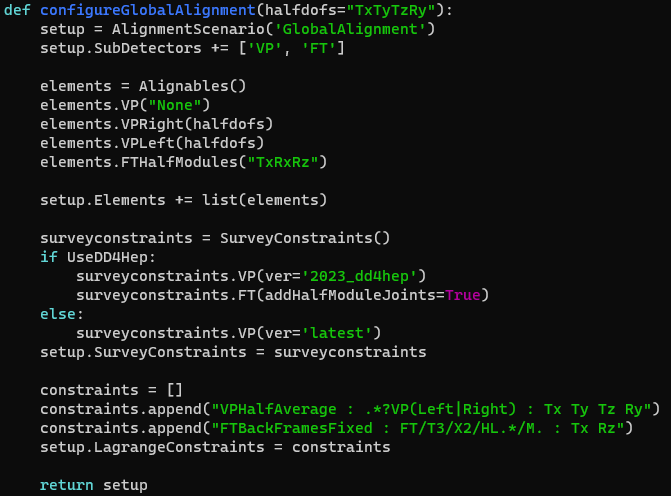
\includegraphics[width=\textwidth]{plots/scenarios.png}
      \end{figure}
    \end{column}
  \end{columns}
\end{frame}

\begin{frame}\frametitle{Alignment configurations}
  \begin{itemize}
    \item v1: SciFi (TxRxRz), no SciFi survey
    \item v2: SciFi (TxRz), no SciFi survey
    \item v3: SciFi (TxRz), SciFi C-Frames survey
    \item v4: SciFi (TxRz), SciFi C-Frames survey, constrain (U|V) layer in T2 for Tx Rz
  \end{itemize}
\end{frame}

\begin{frame}{Global alignment: Tx, Rx vs global z position}
  mean Tx in [mm], Rx in [rad] of each layer
  \begin{columns}
    \begin{column}[c]{0.5\textwidth}
      \begin{figure}
        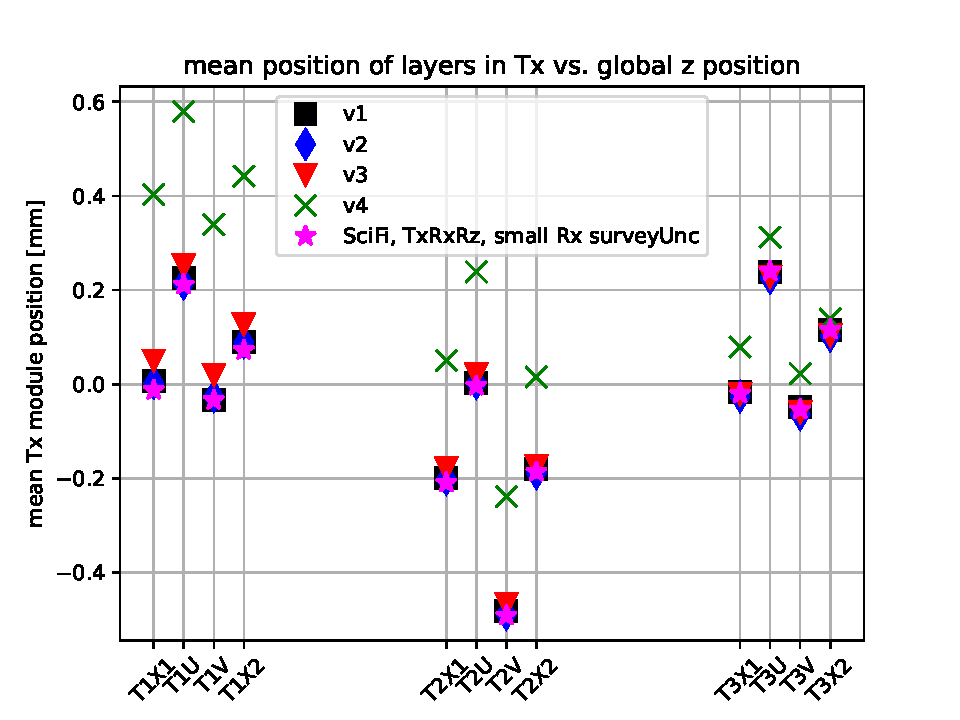
\includegraphics[width=\textwidth]{plots/outfiles_vs_global/all_runs_retest_glob_z_vs_local_Tx.pdf}
      \end{figure}
    \end{column}
    \begin{column}[c]{0.5\textwidth}
      \begin{figure}
        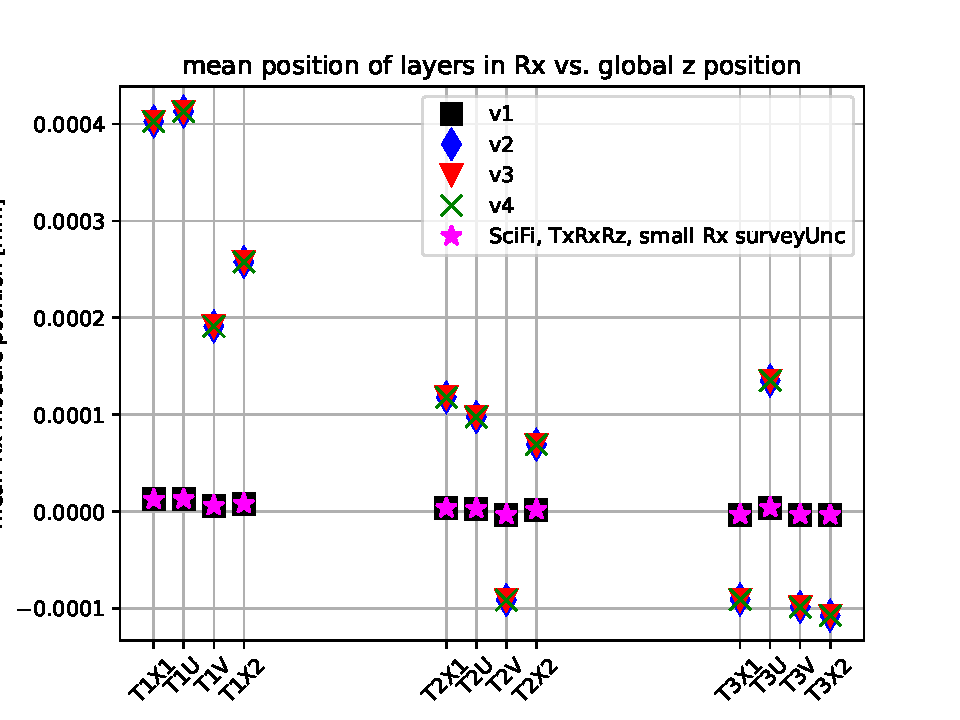
\includegraphics[width=\textwidth]{plots/outfiles_vs_global/all_runs_retest_glob_z_vs_local_Rx.pdf}
      \end{figure}
    \end{column}
  \end{columns}
\end{frame}

\begin{frame}{Global alignment: Ty, Ry vs global z position}
  mean Ty in [mm], Ry in [rad] of each layer
  \begin{columns}
    \begin{column}[c]{0.5\textwidth}
      \begin{figure}
        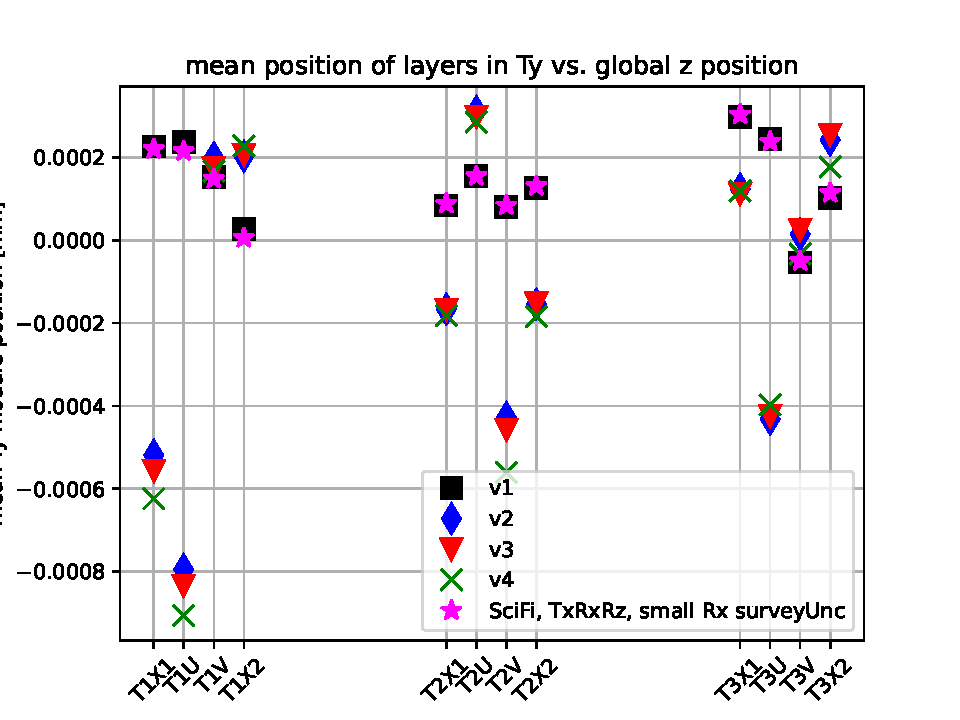
\includegraphics[width=\textwidth]{plots/outfiles_vs_global/all_runs_retest_glob_z_vs_local_Ty.pdf}
      \end{figure}
    \end{column}
    \begin{column}[c]{0.5\textwidth}
      \begin{figure}
        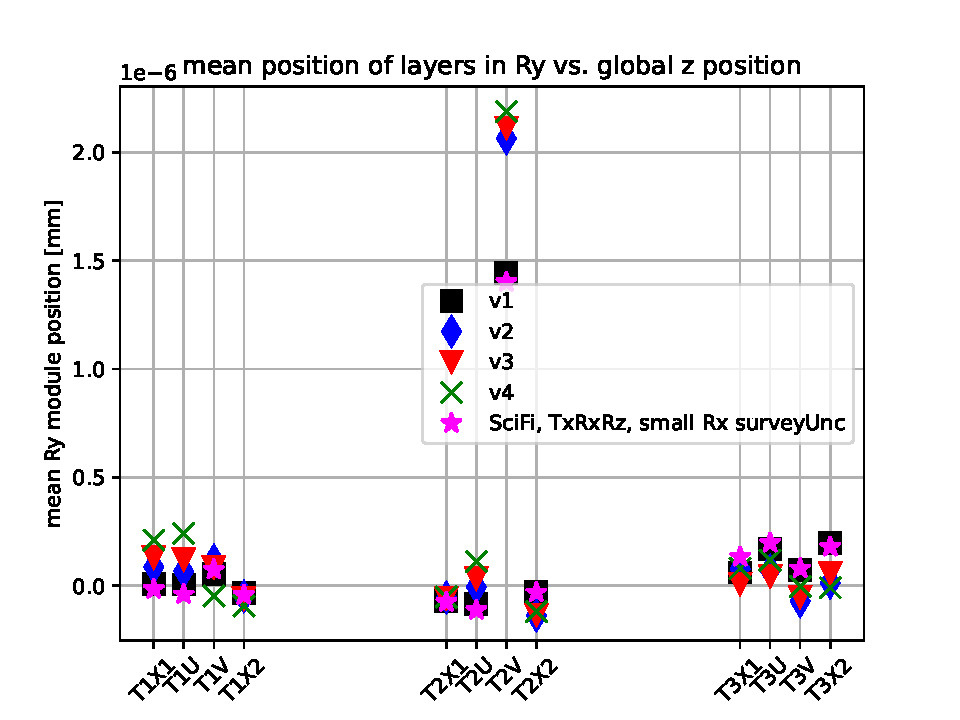
\includegraphics[width=\textwidth]{plots/outfiles_vs_global/all_runs_retest_glob_z_vs_local_Ry.pdf}
      \end{figure}
    \end{column}
  \end{columns}
\end{frame}

\begin{frame}{Global alignment: Tz, Rz vs global z position}
  mean Tz in [mm], Rz in [rad] of each layer
  \begin{columns}
    \begin{column}[c]{0.5\textwidth}
      \begin{figure}
        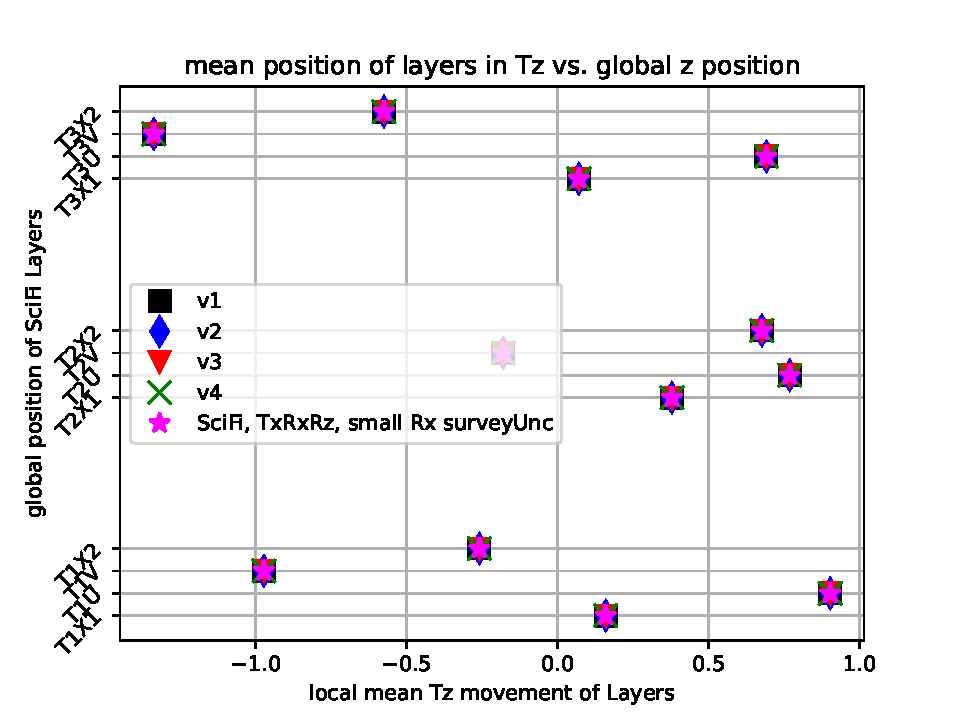
\includegraphics[width=\textwidth]{plots/outfiles_vs_global/all_runs_retest_glob_z_vs_local_Tz.pdf}
      \end{figure}
    \end{column}
    \begin{column}[c]{0.5\textwidth}
      \begin{figure}
        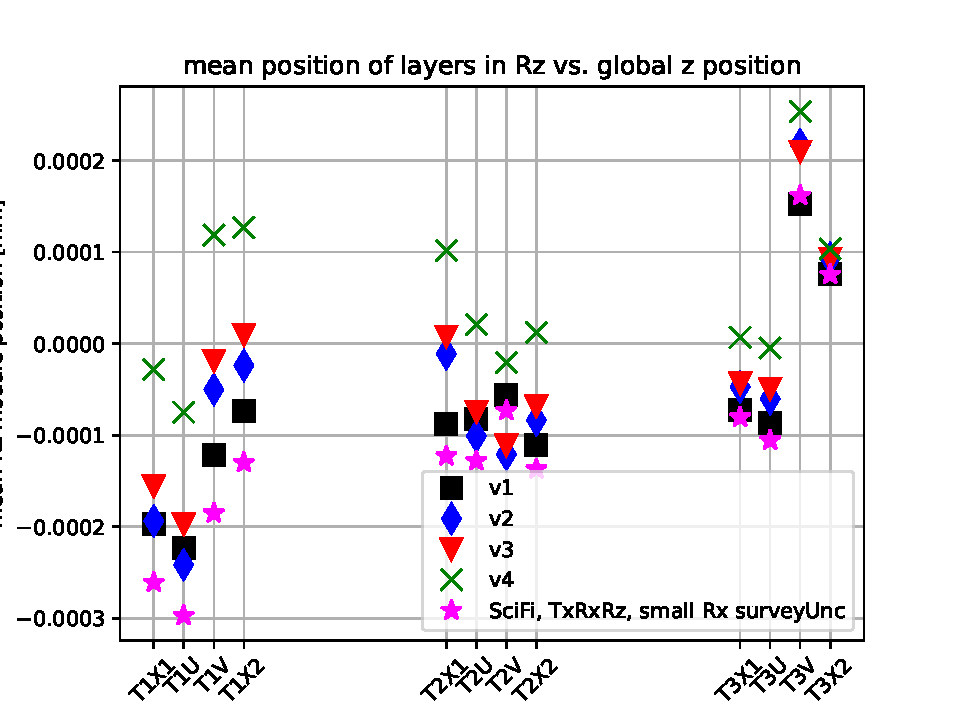
\includegraphics[width=\textwidth]{plots/outfiles_vs_global/all_runs_retest_glob_z_vs_local_Rz.pdf}
      \end{figure}
    \end{column}
  \end{columns}
\end{frame}

\begin{frame}
  \begin{itemize}
    \item without aligning Rx there will be a non-zero Rx; maximum 0.4 mrad
    \item visible but small z-rotation across stations
    \item Tx constraint in v4 shifted everything closer to zero but didn't solve the problem for Tx behaviour
    \item Ty worse when NOT aligning for Rx \to joint constraint or C-Frame survey cannot correct for that
  \end{itemize}
\end{frame}

\begin{frame}{Comparison VELO only vs global constants}
  \begin{columns}
    \begin{column}[c]{0.5\textwidth}
      \begin{figure}
        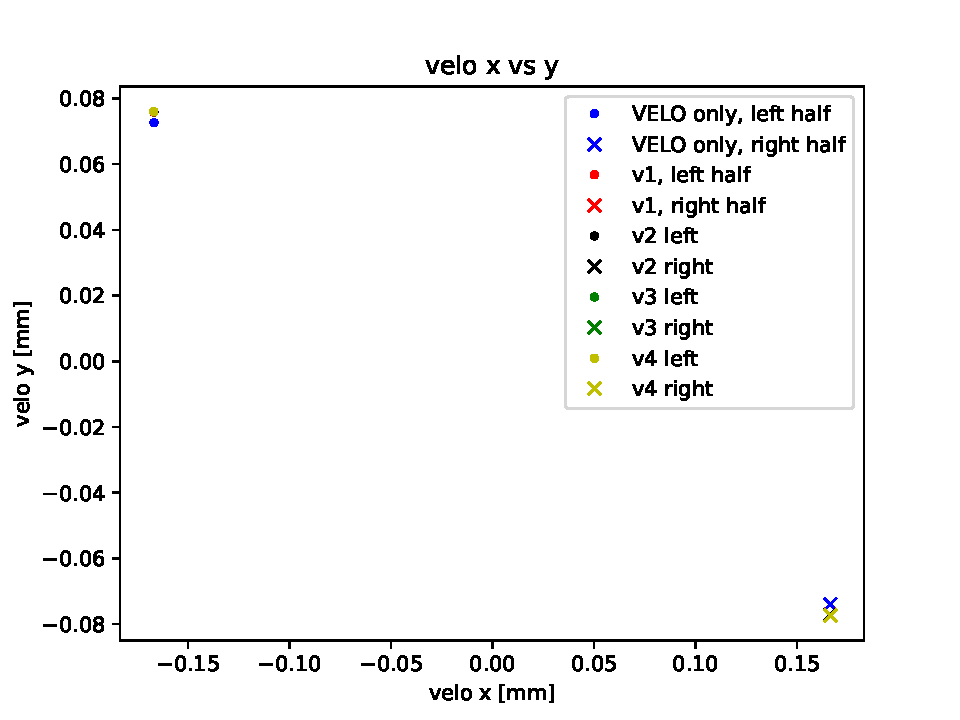
\includegraphics[width=\textwidth]{plots/velo_constants.pdf}
      \end{figure}
    \end{column}
    \begin{column}[c]{0.5\textwidth}
      \begin{itemize}
        \item dots: left velo half; crosses: right velo half
        \item v1 \to v4 nearly identical (on top of each other)
        \item difference between VELO only and from the global alignment: 3.5 $\mu m$
        \item \to is this withing the VELO acceptance or is 3.5 $\mu m$ problematic?
      \end{itemize}
    \end{column}
  \end{columns}
\end{frame}

\begin{frame}{T1 SciFi module constants in global: x vs y}
  \begin{columns}
    \begin{column}[c]{0.5\textwidth}
      \begin{figure}
        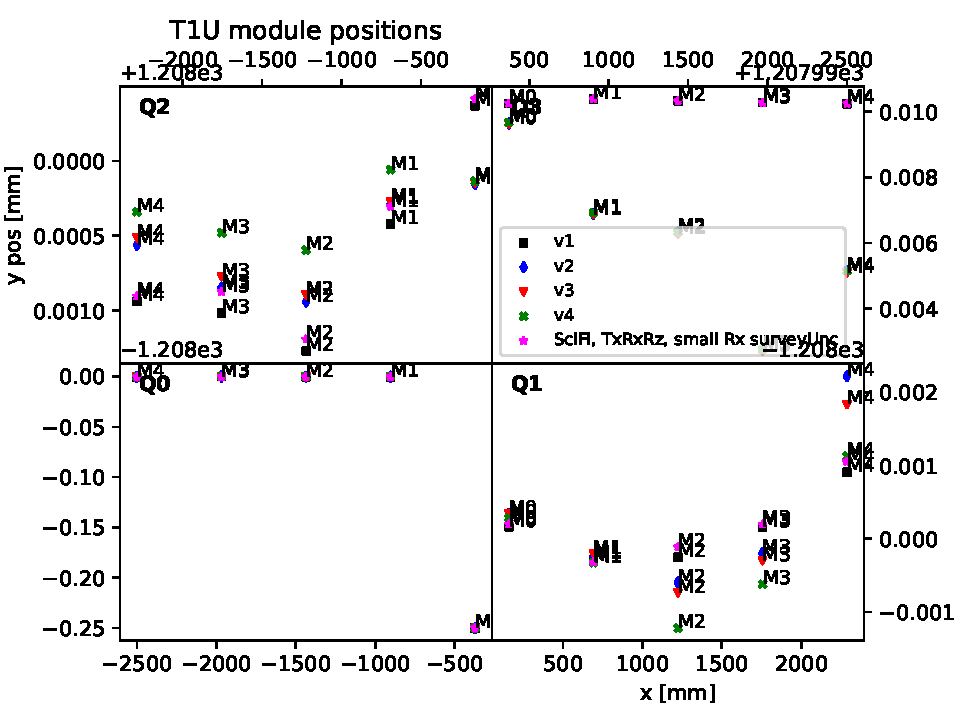
\includegraphics[width=0.61\textwidth]{plots/out_x_y_pos/retest_x_vs_zT1U.pdf}
        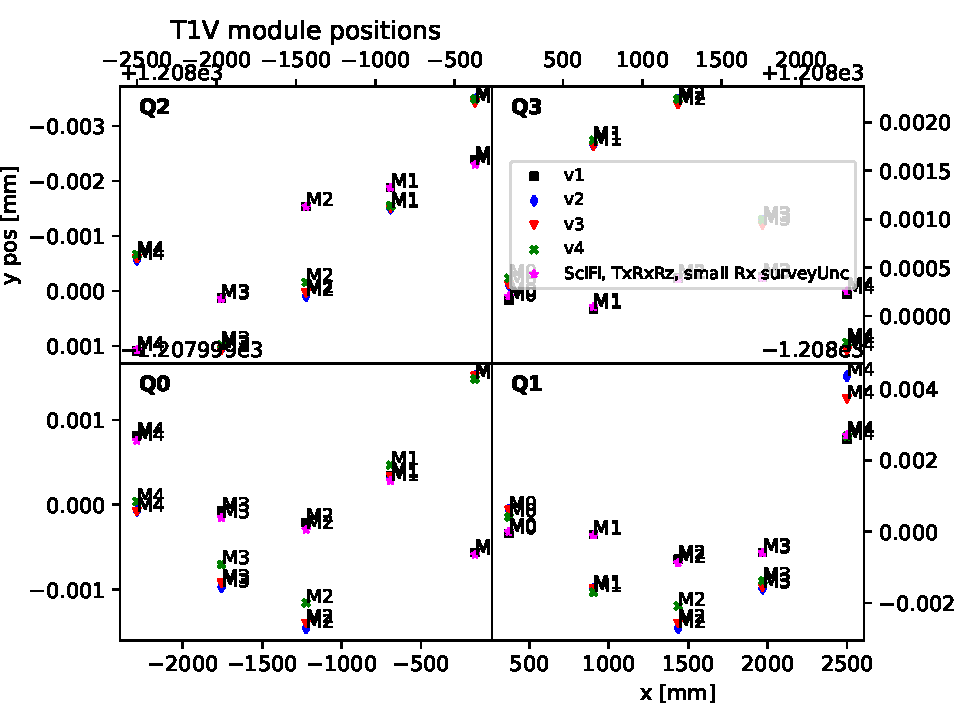
\includegraphics[width=0.61\textwidth]{plots/out_x_y_pos/retest_x_vs_zT1V.pdf}
      \end{figure}
    \end{column}
    \begin{column}[c]{0.5\textwidth}
      \begin{figure}
        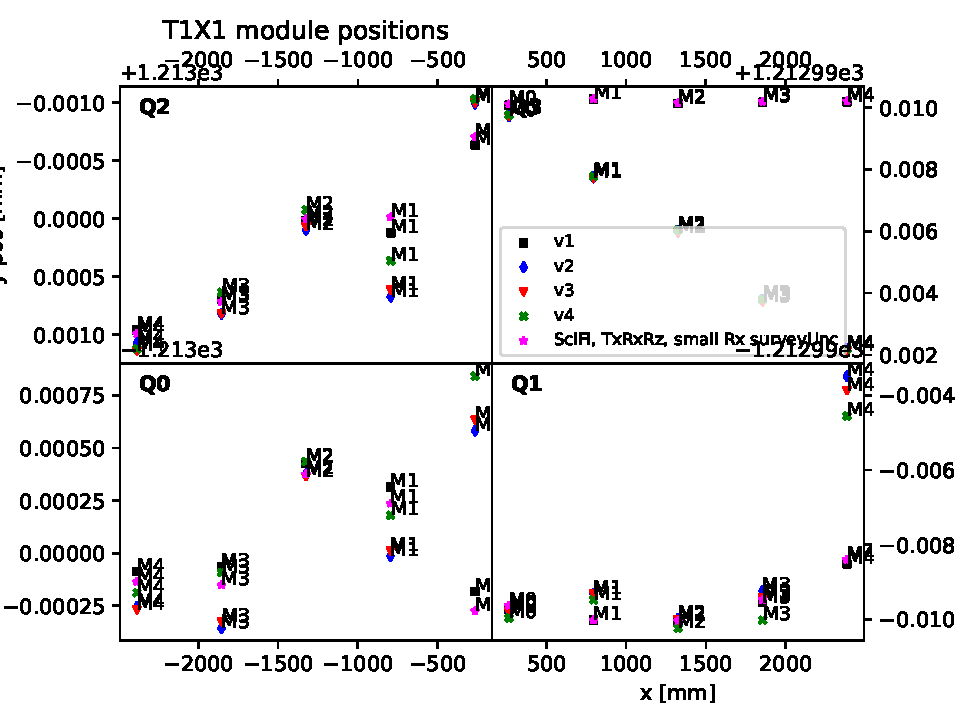
\includegraphics[width=0.61\textwidth]{plots/out_x_y_pos/retest_x_vs_zT1X1.pdf}
        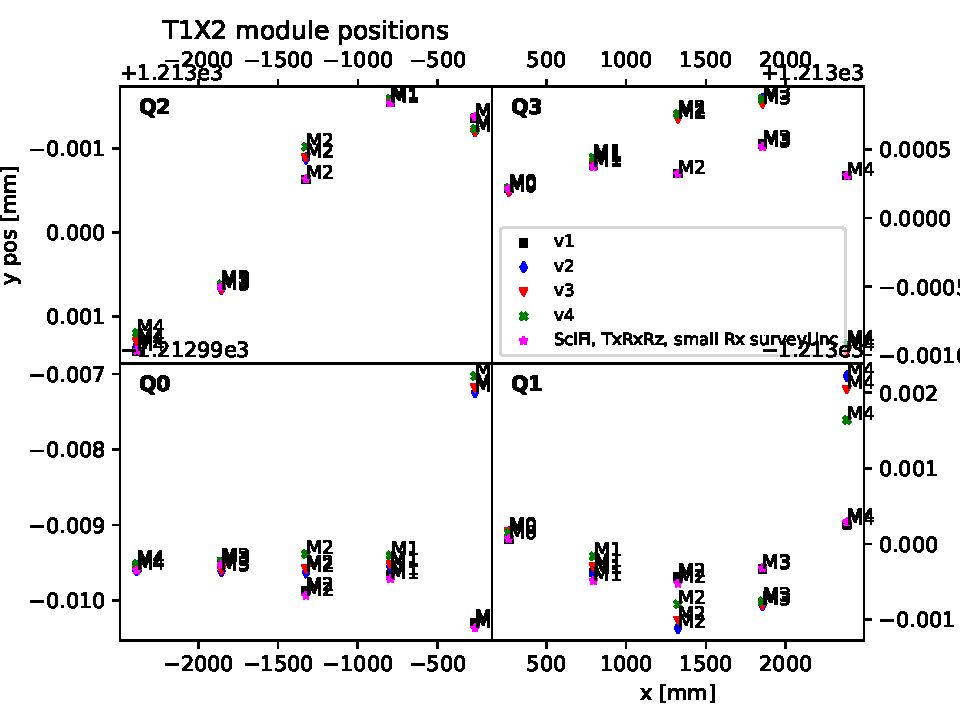
\includegraphics[width=0.61\textwidth]{plots/out_x_y_pos/retest_x_vs_zT1X2.pdf}
      \end{figure}
    \end{column}
  \end{columns}
\end{frame}

\begin{frame}{T2 SciFi module constants in global: x vs y}
  \begin{columns}
    \begin{column}[c]{0.5\textwidth}
      \begin{figure}
        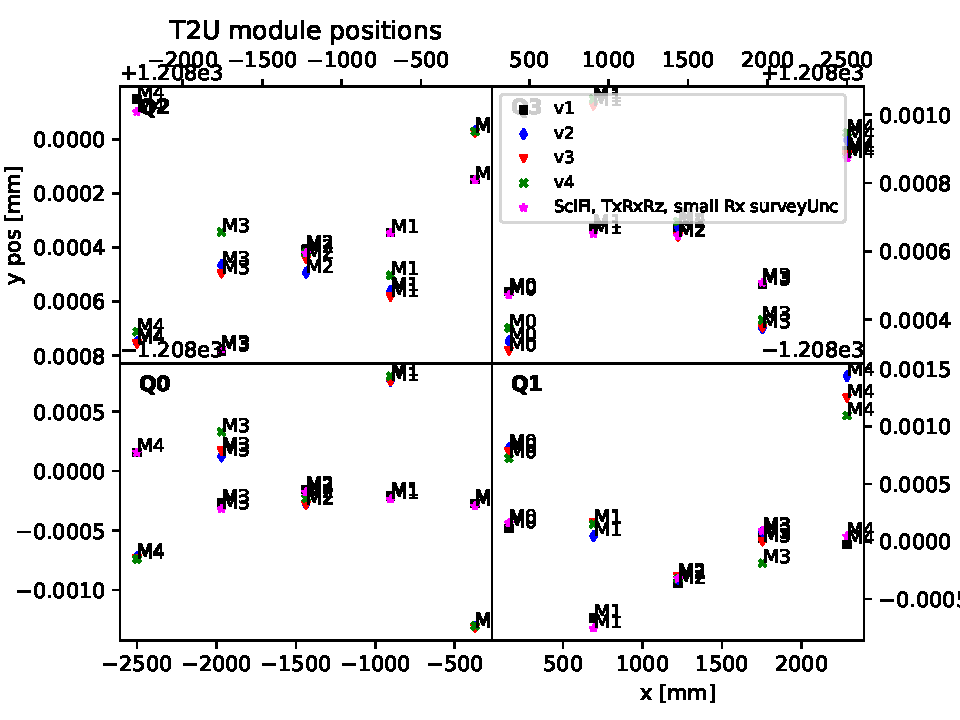
\includegraphics[width=0.61\textwidth]{plots/out_x_y_pos/retest_x_vs_zT2U.pdf}
        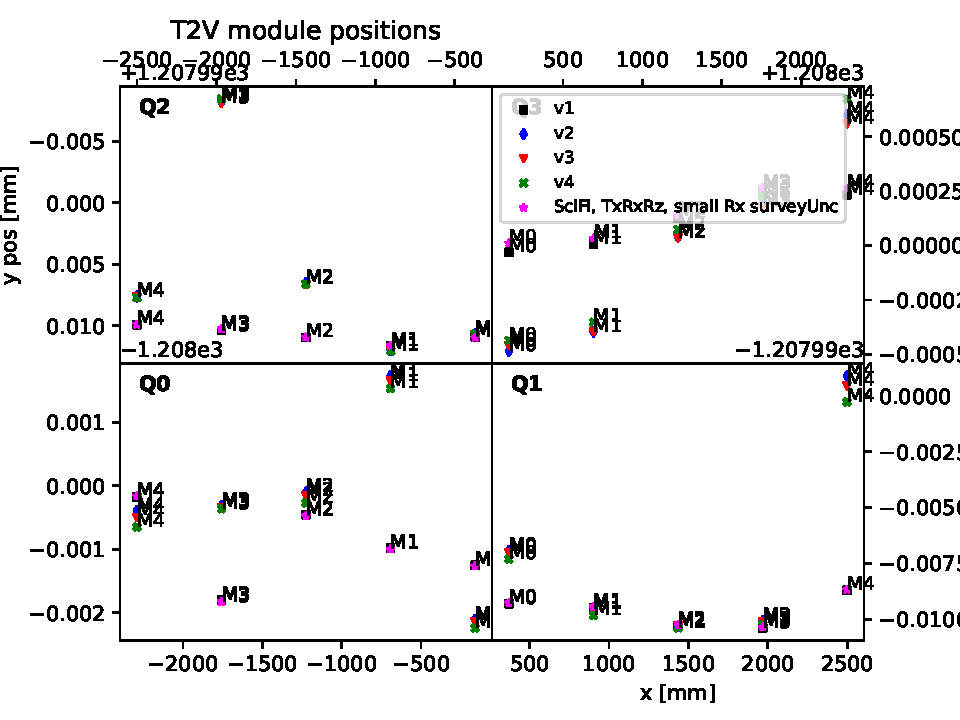
\includegraphics[width=0.61\textwidth]{plots/out_x_y_pos/retest_x_vs_zT2V.pdf}
      \end{figure}
    \end{column}
    \begin{column}[c]{0.5\textwidth}
      \begin{figure}
        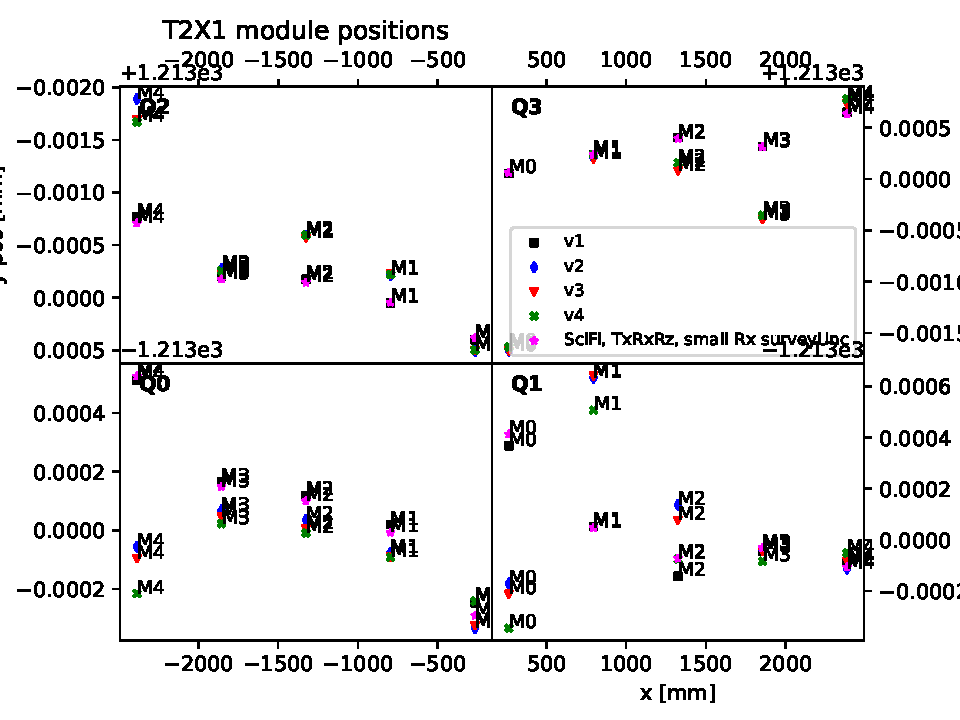
\includegraphics[width=0.61\textwidth]{plots/out_x_y_pos/retest_x_vs_zT2X1.pdf}
        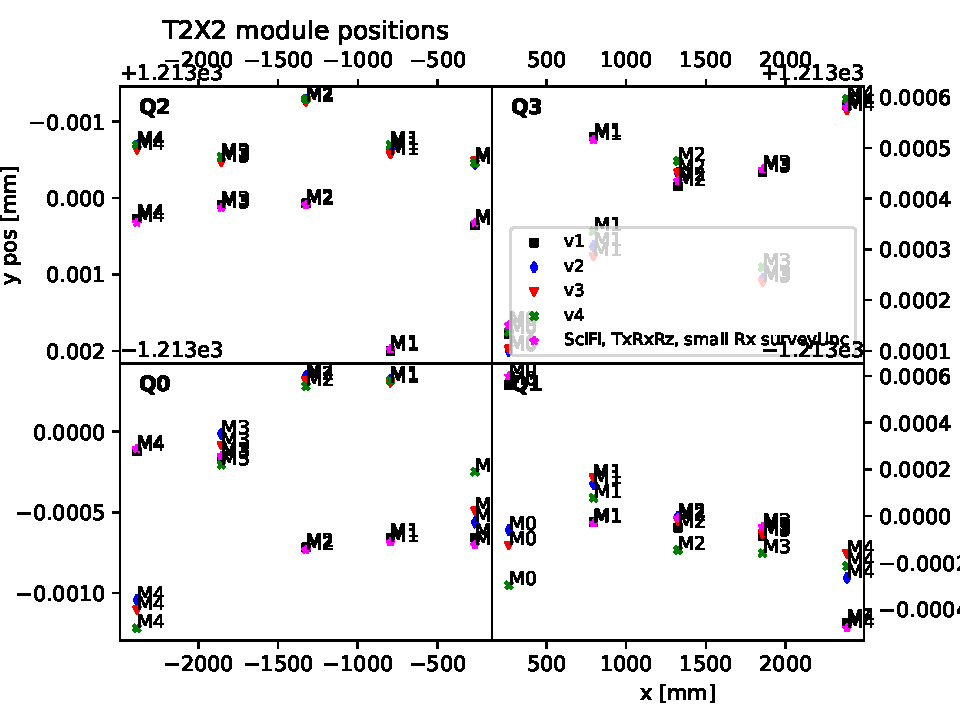
\includegraphics[width=0.61\textwidth]{plots/out_x_y_pos/retest_x_vs_zT2X2.pdf}
      \end{figure}
    \end{column}
  \end{columns}
\end{frame}

\begin{frame}{T3 SciFi module constants in global: x vs y}
  \begin{columns}
    \begin{column}[c]{0.5\textwidth}
      \begin{figure}
        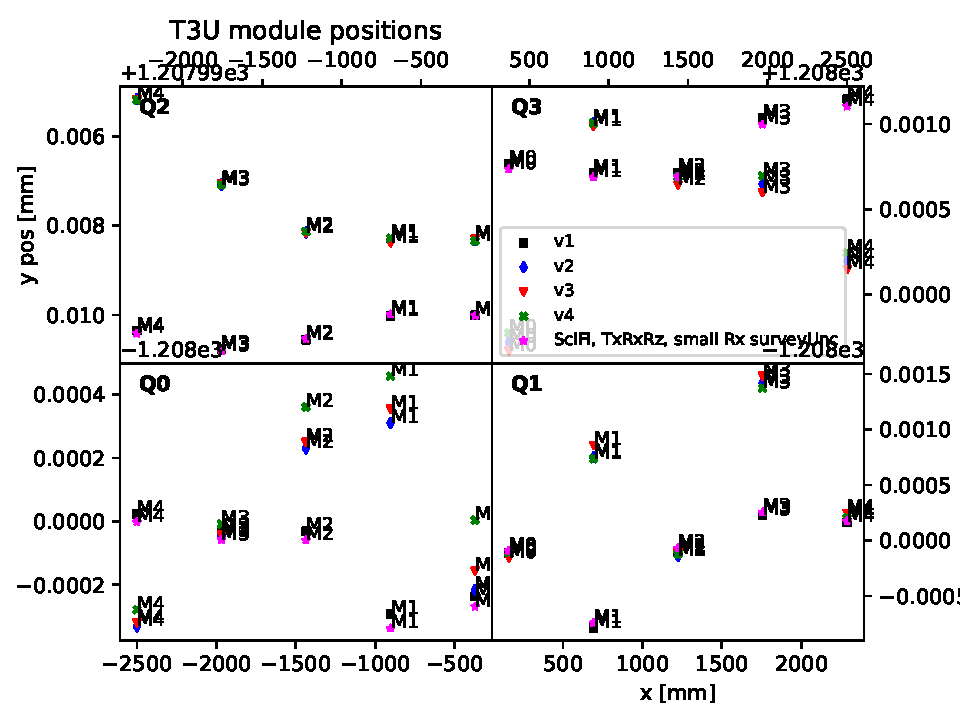
\includegraphics[width=0.61\textwidth]{plots/out_x_y_pos/retest_x_vs_zT3U.pdf}
        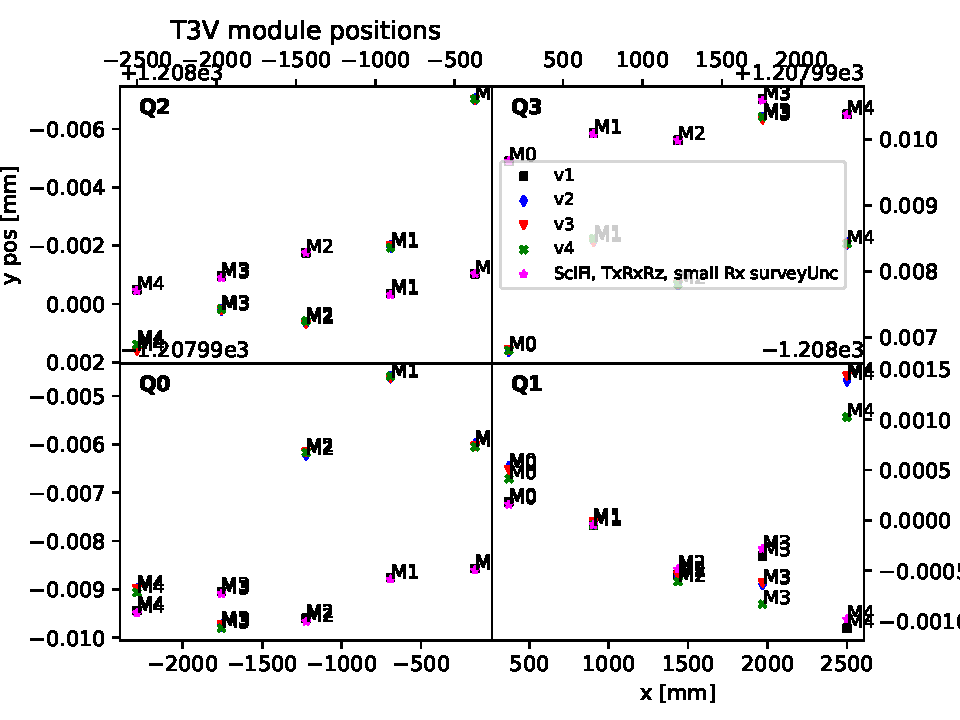
\includegraphics[width=0.61\textwidth]{plots/out_x_y_pos/retest_x_vs_zT3V.pdf}
      \end{figure}
    \end{column}
    \begin{column}[c]{0.5\textwidth}
      \begin{figure}
        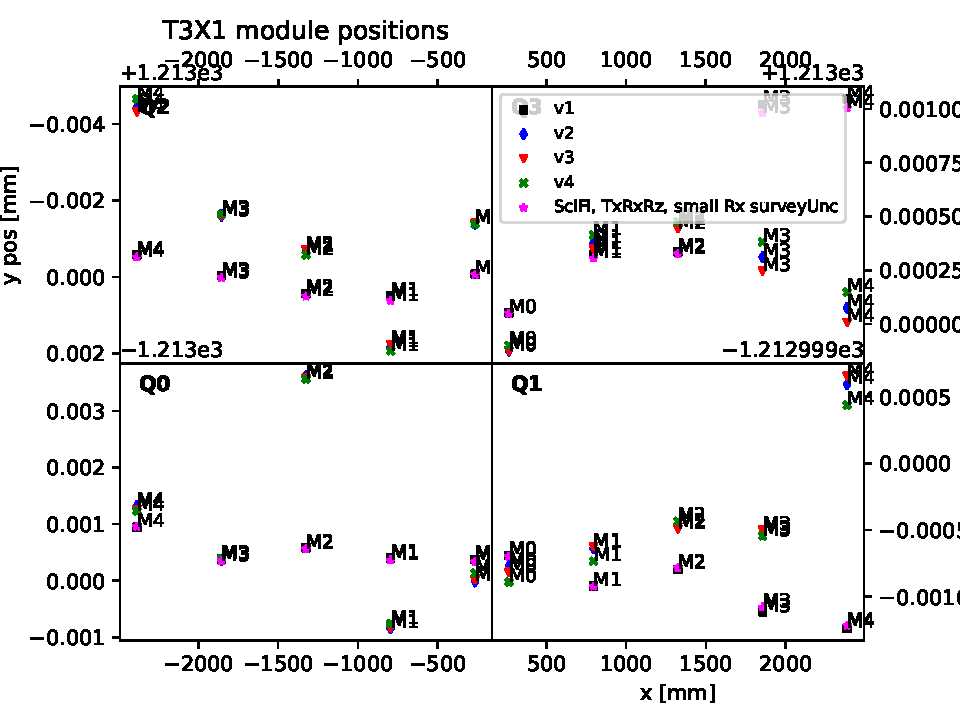
\includegraphics[width=0.61\textwidth]{plots/out_x_y_pos/retest_x_vs_zT3X1.pdf}
        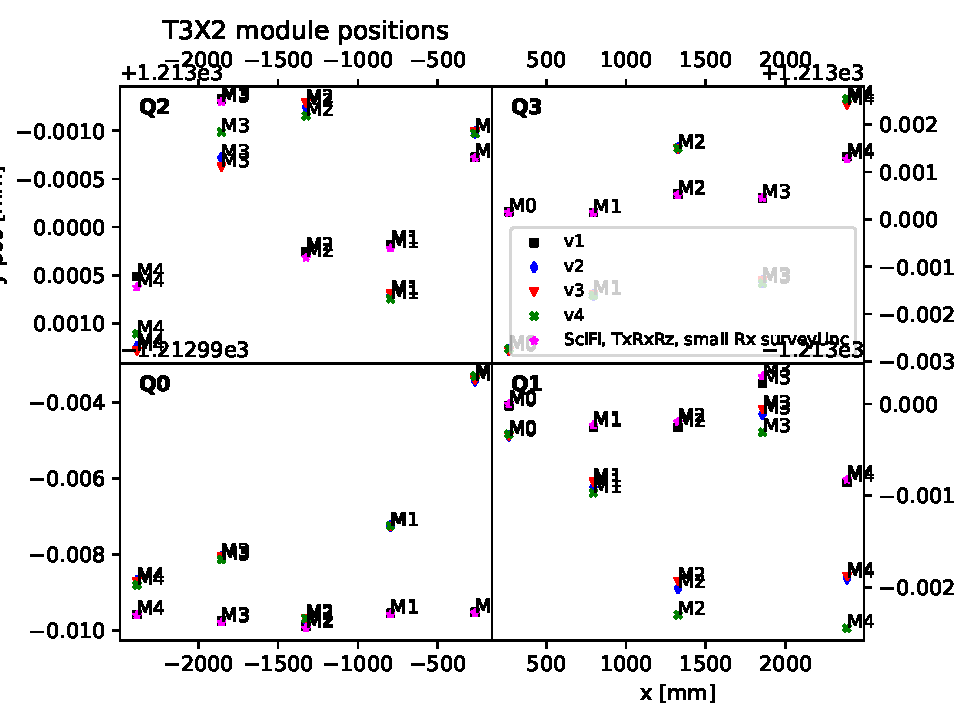
\includegraphics[width=0.61\textwidth]{plots/out_x_y_pos/retest_x_vs_zT3X2.pdf}
      \end{figure}
    \end{column}
  \end{columns}
\end{frame}

\begin{frame}{T1 SciFi module constants in local: x vs y}
  \begin{columns}
    \begin{column}[c]{0.5\textwidth}
      \begin{figure}
        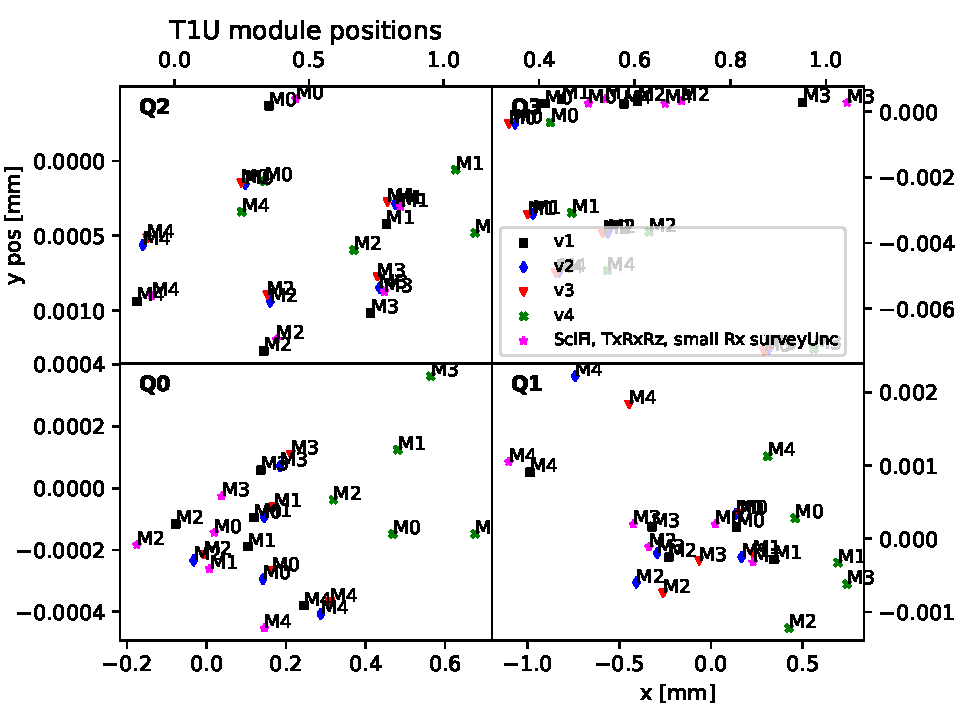
\includegraphics[width=0.61\textwidth]{plots/out_x_y_pos/retest_x_vs_y_local_T1U.pdf}
        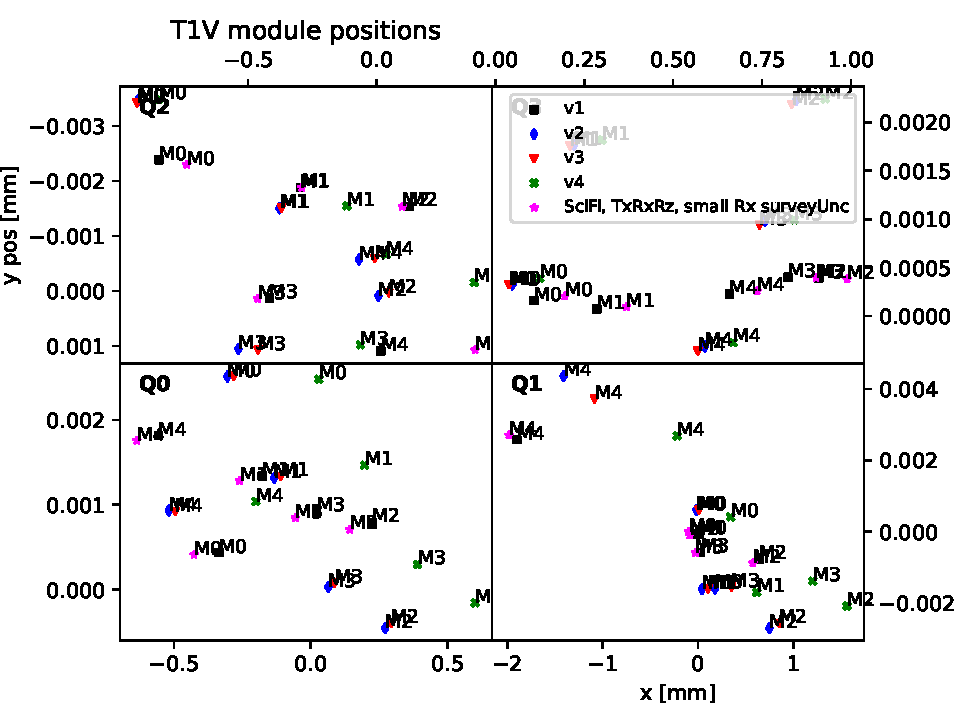
\includegraphics[width=0.61\textwidth]{plots/out_x_y_pos/retest_x_vs_y_local_T1V.pdf}
      \end{figure}
    \end{column}
    \begin{column}[c]{0.5\textwidth}
      \begin{figure}
        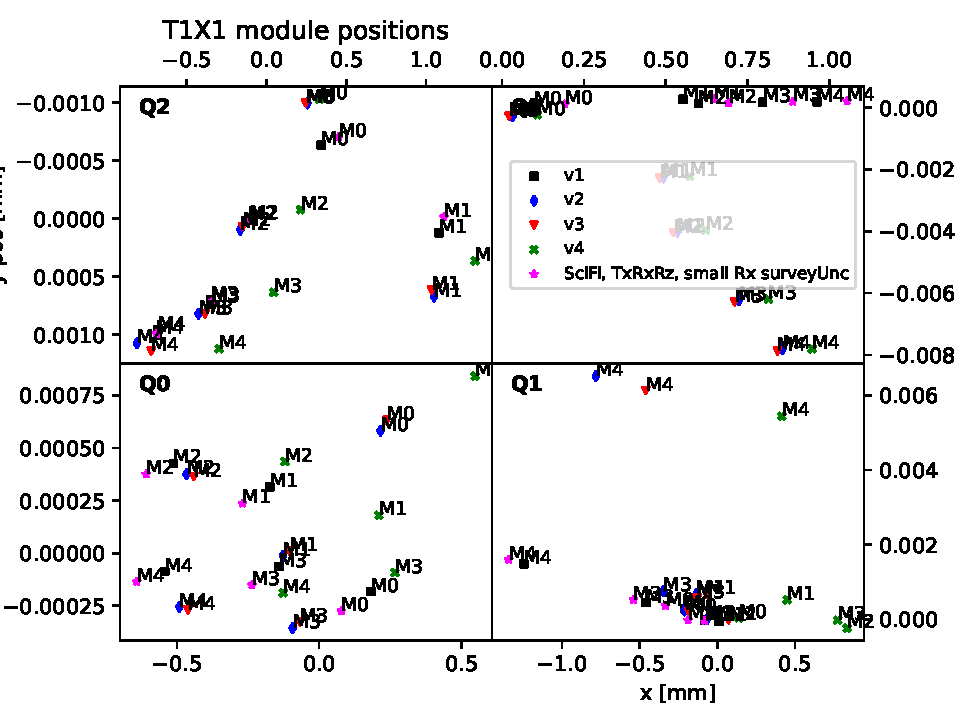
\includegraphics[width=0.61\textwidth]{plots/out_x_y_pos/retest_x_vs_y_local_T1X1.pdf}
        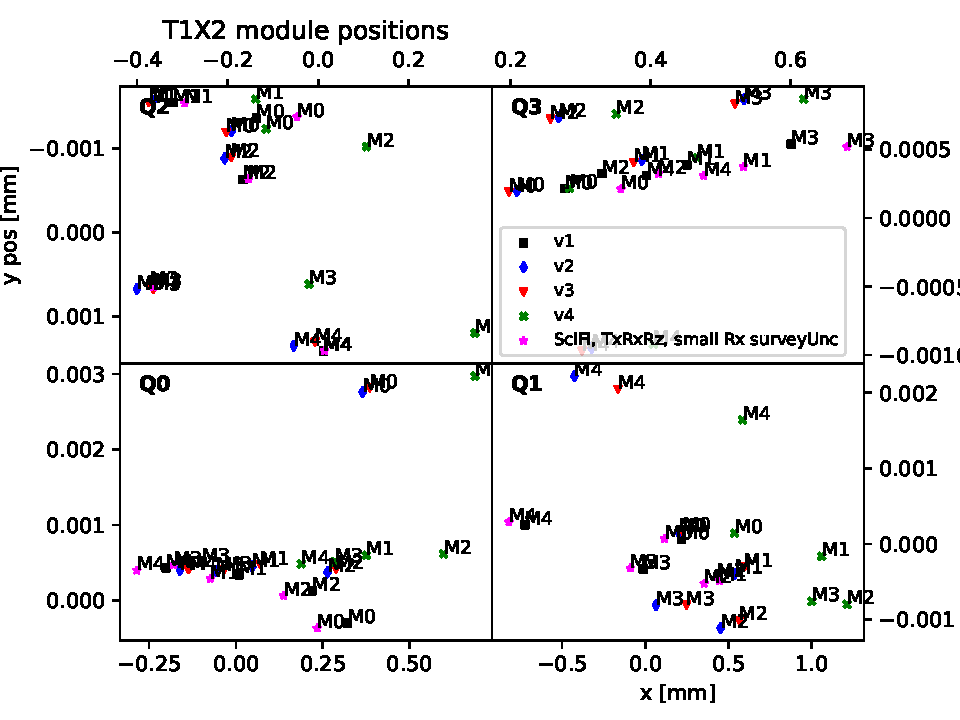
\includegraphics[width=0.61\textwidth]{plots/out_x_y_pos/retest_x_vs_y_local_T1X2.pdf}
      \end{figure}
    \end{column}
  \end{columns}
\end{frame}

\begin{frame}{T2 SciFi module constants in local: x vs y}
  \begin{columns}
    \begin{column}[c]{0.5\textwidth}
      \begin{figure}
        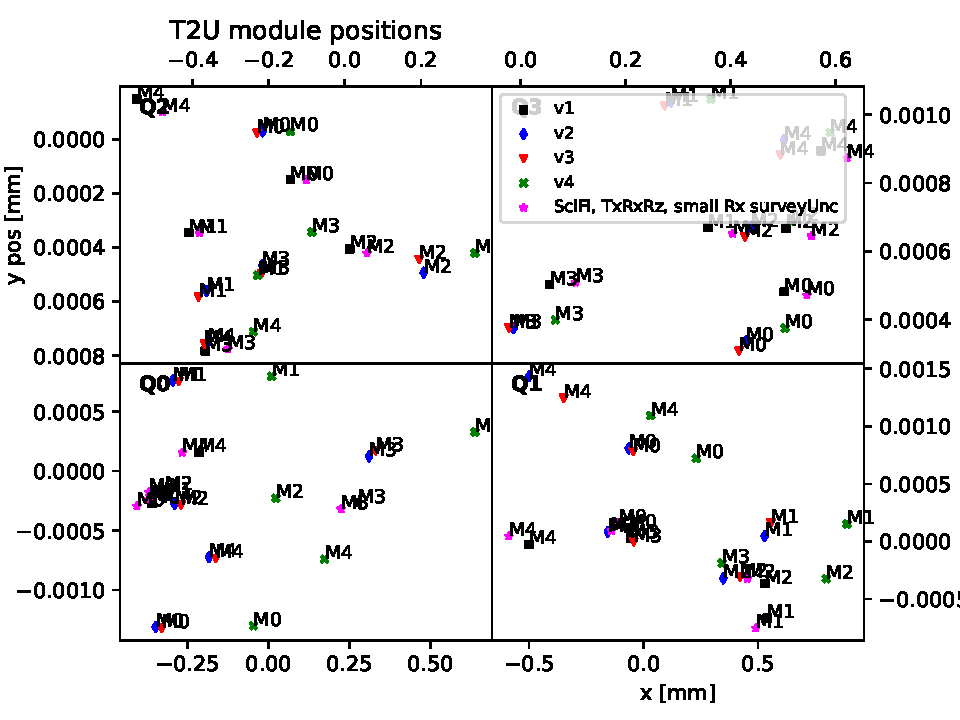
\includegraphics[width=0.61\textwidth]{plots/out_x_y_pos/retest_x_vs_y_local_T2U.pdf}
        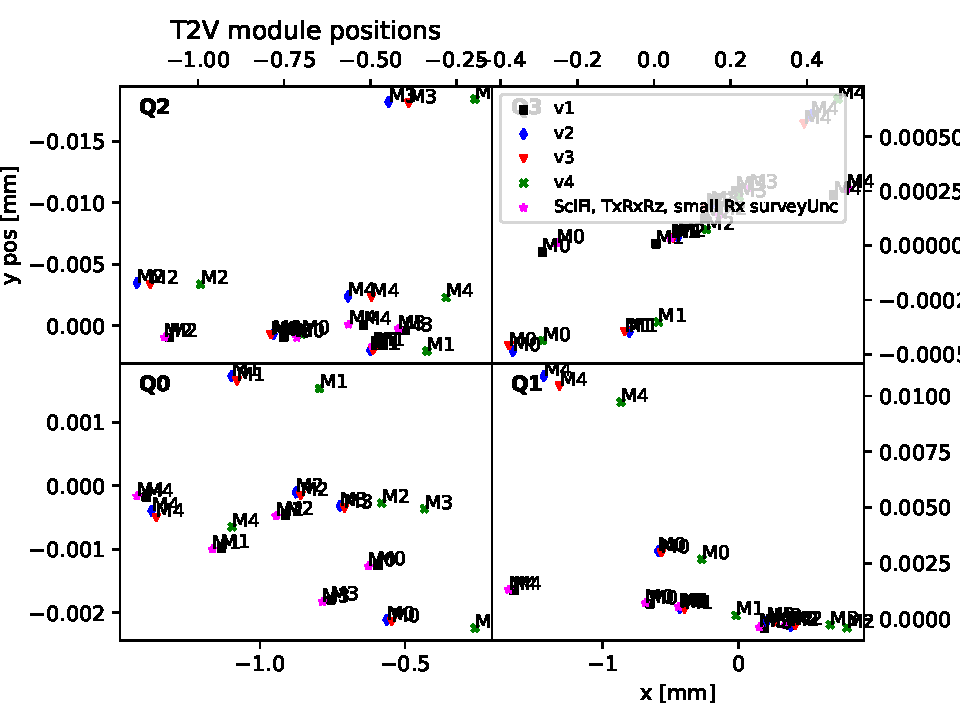
\includegraphics[width=0.61\textwidth]{plots/out_x_y_pos/retest_x_vs_y_local_T2V.pdf}
      \end{figure}
    \end{column}
    \begin{column}[c]{0.5\textwidth}
      \begin{figure}
        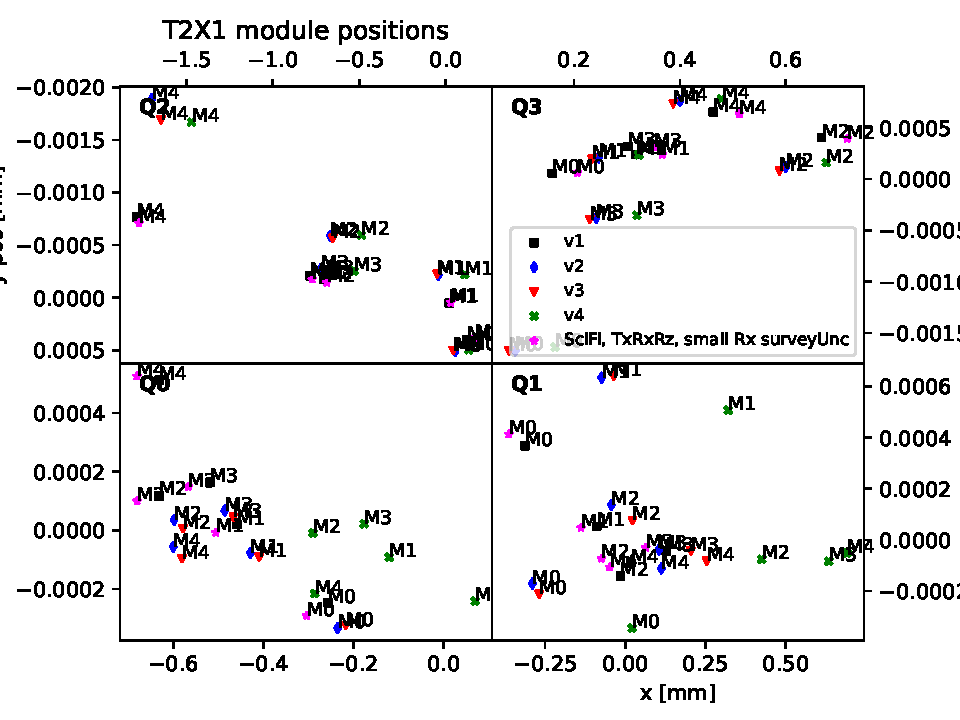
\includegraphics[width=0.61\textwidth]{plots/out_x_y_pos/retest_x_vs_y_local_T2X1.pdf}
        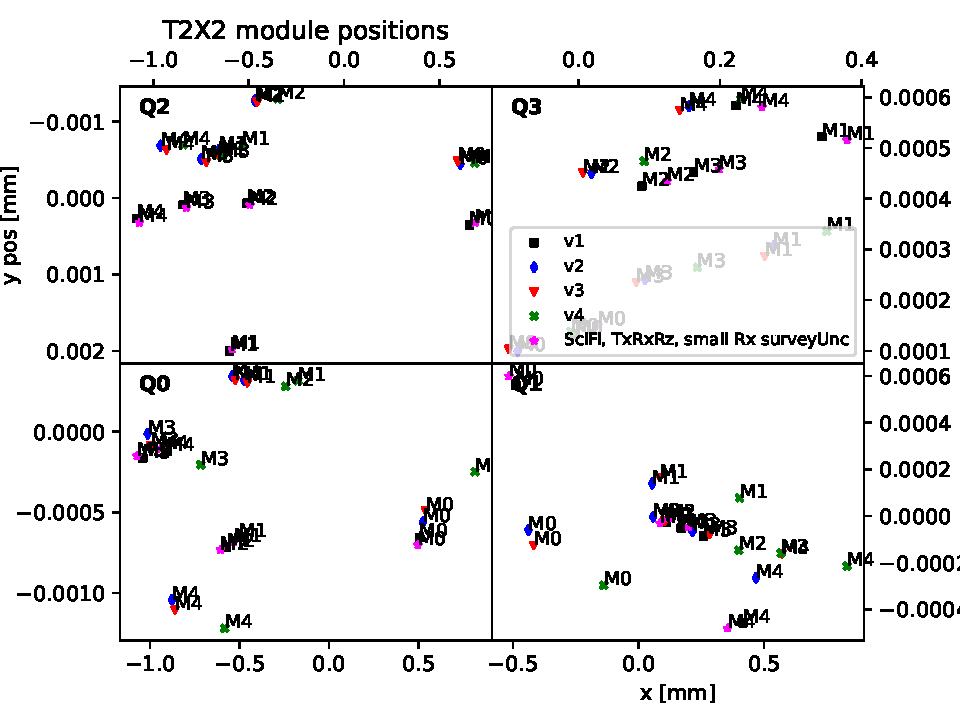
\includegraphics[width=0.61\textwidth]{plots/out_x_y_pos/retest_x_vs_y_local_T2X2.pdf}
      \end{figure}
    \end{column}
  \end{columns}
\end{frame}

\begin{frame}{T3 SciFi module constants in local: x vs y}
  \begin{columns}
    \begin{column}[c]{0.5\textwidth}
      \begin{figure}
        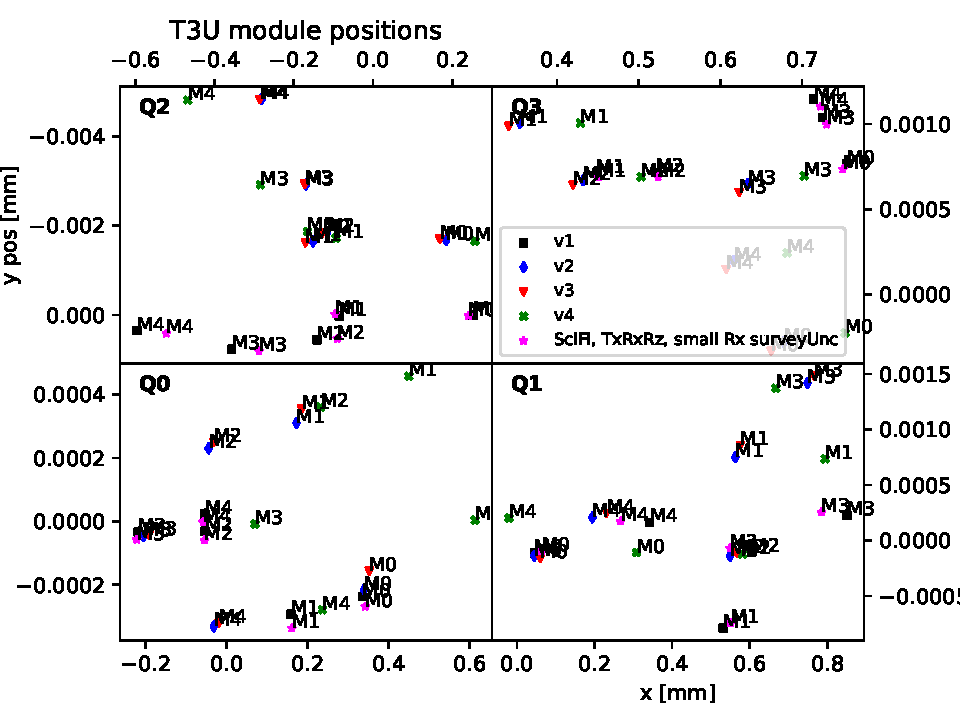
\includegraphics[width=0.61\textwidth]{plots/out_x_y_pos/retest_x_vs_y_local_T3U.pdf}
        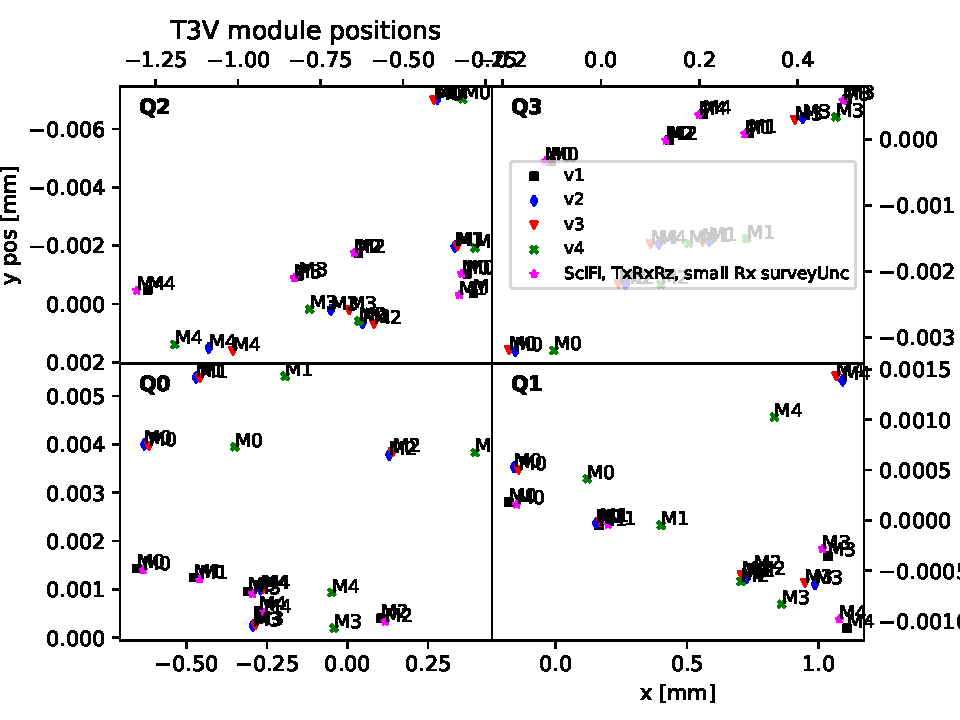
\includegraphics[width=0.61\textwidth]{plots/out_x_y_pos/retest_x_vs_y_local_T3V.pdf}
      \end{figure}
    \end{column}
    \begin{column}[c]{0.5\textwidth}
      \begin{figure}
        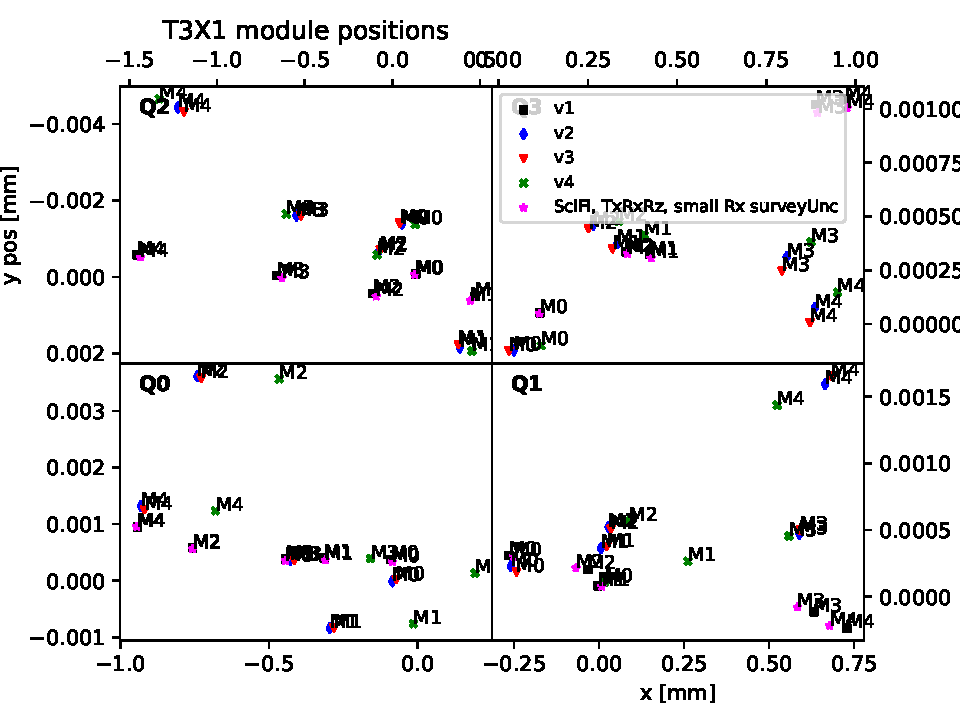
\includegraphics[width=0.61\textwidth]{plots/out_x_y_pos/retest_x_vs_y_local_T3X1.pdf}
        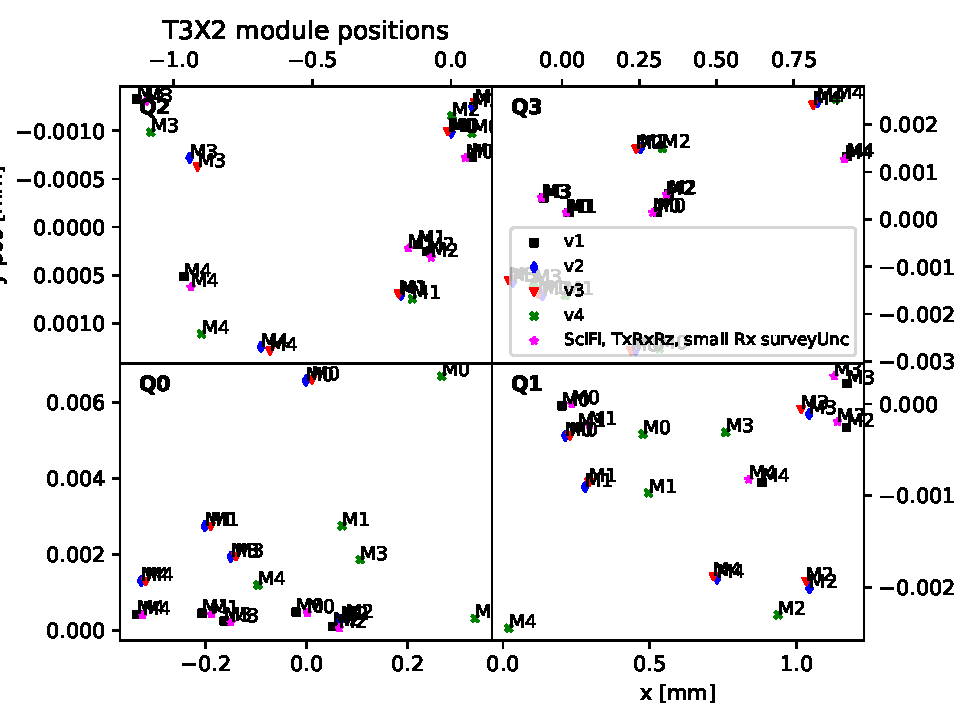
\includegraphics[width=0.61\textwidth]{plots/out_x_y_pos/retest_x_vs_y_local_T3X2.pdf}
      \end{figure}
    \end{column}
  \end{columns}
\end{frame}

\begin{frame}{module edge difference in y direction}
  \begin{columns}
    \begin{column}[c]{0.6\textwidth}
      \begin{figure}
        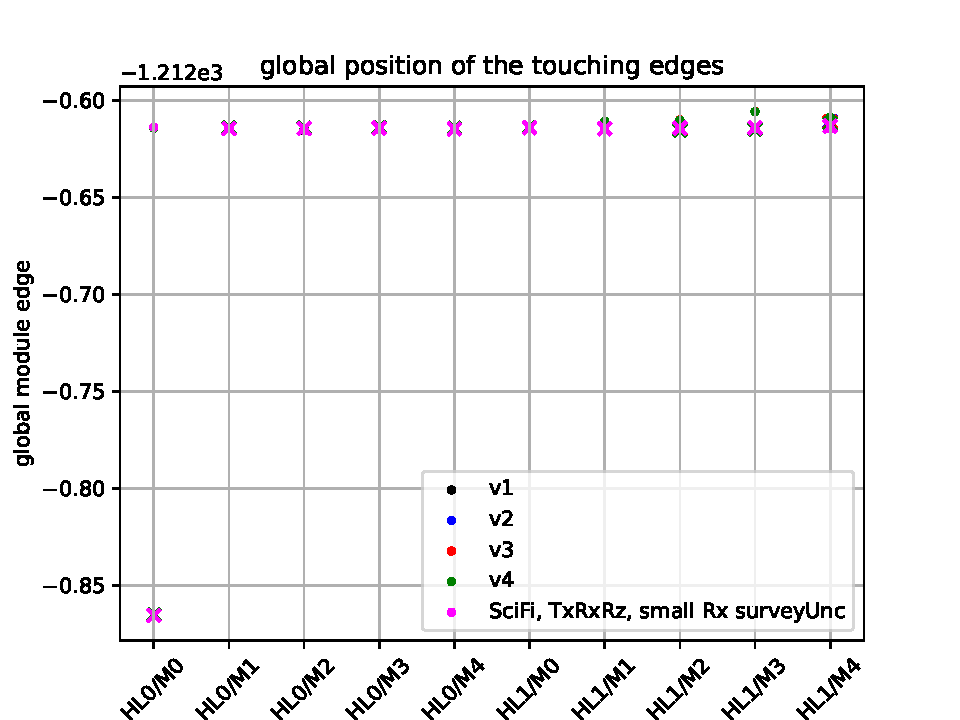
\includegraphics[width=0.5\textwidth]{plots/out_x_y_pos/retest_global_alignT1U.pdf}
        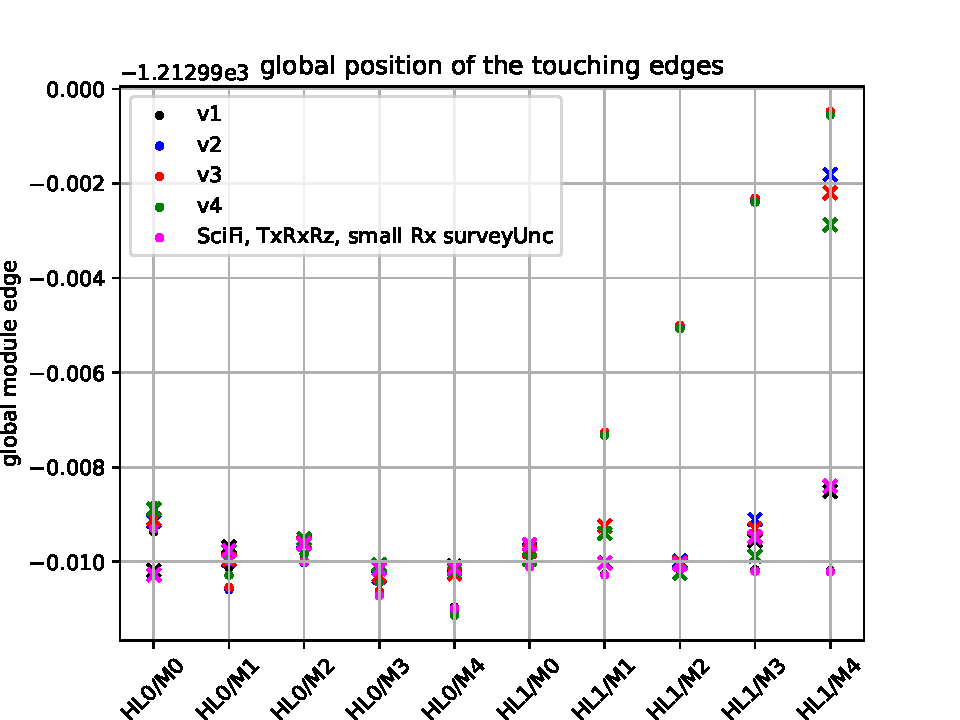
\includegraphics[width=0.5\textwidth]{plots/out_x_y_pos/retest_global_alignT1X1.pdf}
      \end{figure}
    \end{column}
    \begin{column}[c]{0.4\textwidth}
      \begin{itemize}
        \item dots: middle edge of top half module, cross: middle edge of bottom half module
        \item joints uncertainties: 0.01 0.0012 0.0019 0.0004 0.0002 0.00017
        \item \to half modules fairly close everywhere, but T1UQ0M0
        \item T1X1: Q1 is drifting from Q3
      \end{itemize}
    \end{column}
  \end{columns}
\end{frame}

\end{document}
